
\section{Enumerative Combinatorics}

$A$ finite set, $|A|$ = ?

$(A_n)_{n ≥ 0}$ system of finite sets, $a_n = |A_n|$, what is the \dt{counting sequence} $(a_n)_{n ≥ 0}$

The goal might be to find
\begin{compactitem}
  \item a closed formula (often impossible),
  \item a recursion,
  \item a generating function (e.g. $\sum_{n \geq 0}[a_n z^n]$),
  \item asymptotic estimates, $a_n$ symptotically similar to $b_n$:\\
    $a_n \sim b_n \iff \lim_{n \to \infty} \frac{a_n}{b_n} = 1$
\end{compactitem}


\textbf{Example.}
\begin{align*}
  A_n &= \{\text{permutations of } 1,2, \ldots, n\}, |A_n| = n! \\
  a_1 &= 1, a_n = n a_{n-1} \\
  a_n &\sim \left(\frac{n}{e} \right)^n \sqrt{2\pi n}
\end{align*}


\subsection{Counting principles}

Elementary counting principles:
% TODO make subsubsections out of this
\begin{compactenum}
  \item Sum principle:
    $A\cap B = \varnothing \implies |A\cup B| = |A| + |B|$
  \item Product principle:
    $|A\times B| = |A| * |B|$
  \item Bijection principle:
    $f: A\mapsto B, \text{bijective}\implies |A| = |B|$
\end{compactenum}

\textbf{Example.}
What is the number of two-digit positive integers?
$|\{10,\ldots,99\}| = 90$

\begin{gather*}
  xy, \quad x\in X=\{1,2,\ldots ,9\}, y\in Y = \{0,1,\ldots ,9\} \\
  |X\times Y| = |X| \cdot |Y| = 9\cdot 10 = 90
    \qquad\text{(product principle)}
\end{gather*}

\textbf{Example.}
We choose a password between 4 and 10 digits. How large is the number of possible passwords?
\begin{align*}
  A_i &&& \text{set of passwords with $i$ digits} \\
  Y &= \{0,1,\ldots ,9\} \\
  A_i &= Y^i, |Y| = 10 \\
  |A_i| &= {10}^i  && \text{(product principle)} \\
  \text{total number} &= 10^4 + 10^5 + \ldots + 10^{10} && \text{(sum principle)}
\end{align*}

\textbf{Example.}
There is a Thief, which saw me using a bank-card, and afterwards stole this card. He saw the code starts with $0$ and contains an $8$. How large is the number of possible passwords?

4 Digits ($0 \ldots$), with the product principle we get $10^3$ options.

Using the sum principle we can subtract the number of codes which do not contain the digit $8$.
\begin{align*}
|A| &= \text{\# possibilities} \\
    &= \underbrace{|A\cup B| - |B|}_{\text{(sum principle, reversed)}} \\
    &= {10}^3 - \text{\# codes not containing 8} \\
    &= {10}^3 - 9^3 = 271.
\end{align*}

\textbf{Example.}
Take a set $A = \{a_1, a_2, \ldots , a_n\}$ and its power set $2^A = \{X \mid X
\subseteq A\}$. $|2^A| = ?$

\begin{align*}
  B &\subseteq A \\
  i_k &\quad\text{indices chosen from A} \\
  B &=\{a_{i_1}, a_{i_2},\ldots, a_{i_k}\} \\
  k &\leq n, 1 \leq i_1 < i_2 < \ldots i_k \leq n
    B &\mapsto
    (b_1, b_2 \ldots  b_n) \in \{0,1\}^n \\
  b_i &=
  \begin{cases}
    1 & a_i\in B \\
    0 & a_i\not\in B
  \end{cases} \\
  f: 2^A &\mapsto \{0,1\}^n &&\text{bijective mapping} \\
  |2^A| &= |\{0, 1\}^n| = 2^n
    &&\text{(bijection principle)} \\
\end{align*}

\subsubsection{Double counting}
If:
\begin{align*}
  A &= \{a_1,a_2,\ldots,a_m\} \\
  B &= \{b_1,b_2,\ldots,b_n\} \\
  R & \subseteq A \times B \\
  \text{Set } R_{i,0} &= \{b \in B \mid a_i\operatorname{R} b\}  && \text{(subscript 0 just means}\\
  \text{Set } R_{0,i} &= \{ a \in A \mid a\operatorname{R} b_i \}  && \text{that this part is fixed)}
\end{align*}


%Set R_{i,0} = \{b \in B \mid (a_i,b) \in R\}
Then:
\begin{align*}
  |R| &= \sum_{i=1}^m |R_{i,0}|\\
    &= \sum_{j=1}^n |R_{0,j}|
\end{align*}

\textbf{Proof.}
Define matrix $(x_{ij})_{i = 1,\ldots,m; j = 1,\ldots ,n}$ with

\[x_{ij} = \begin{cases}
    1 & a_i\operatorname{R} b_j \\
    0 &\text{otherwise}
  \end{cases}
\]

The first sum is the row-wise sum, the second sum column-wise. Of course, summing up all the elements of the matrix, you get the same result. In some problems, this equivalence may be helpful, because one of the sums is easier to compute than the other.


\textbf{Example.}
\begin{align*}
  \tau(n) &= \text{average number of divisors of an integer k}, 1 ≤ k ≤ n \\
  d(n) &= \text{ number of divisors of n} \\
  \tau(n) &= \frac{d(1)+\ldots+d(n)}{n} \\
    &= \frac1n\sum_{i=1}^n d(i)
\end{align*}

\bigskip
\begin{table}[H]
  \begin{center}
    \begin{tabular}{r|ccccccccc}
      \toprule
      $n$    &1&2&3&4&5&6&7&8&9 \\
      $d(n)$ &1&2&2&3&2&4&2&4&3 \\
      \bottomrule
    \end{tabular}
    \caption{The number of divisors for every number from $1$ to $9$. $\text{E.g.: } n = 6, \tau(6) = \frac{7}{3}$}
  \end{center}
\end{table}

\begin{align*}
  A &= B = \{1,\ldots,n\} \\
  R & \subseteq A\times B :\ a\operatorname{R} b\iff a|b && \text{ ($a$ divides $b$)}
\end{align*}
\bigskip

One may write down $\operatorname{R}$ as a matrix:

\begin{table}[H]
  \begin{center}
    \begin{tabular}{l|cccccc}
      & \textbf{1} & \textbf{2} & \textbf{3} & \textbf{4} & \textbf{5} & \textbf{6} \\
      \hline \textbf{1} & 1 & 1 & 1 & 1 &  1 & 1 \\
      \textbf{2} & 0 & 1 & 0 & 1 &  0 & 1 \\
      \textbf{3} & 0 & 0 & 1 & 0 &  0 & 1 \\
      \textbf{4} & 0 & 0 & 0 & 1 &  0 & 0 \\
      \textbf{5} & 0 & 0 & 0 & 0 &  1 & 0 \\
      \textbf{6} & 0 & 0 & 0 & 0 &  0 & 1
    \end{tabular}
    \caption{Table of relations ``a divides b'' for the numbers 1 to 6.}
  \end{center}
\end{table}

\begin{align*}
  \text{$n$ prime}
    &\implies d(n) = 2 \\
  n = p^e, p\in \mathbb{P}, e\in \mathbb{N}^{+}
    &\implies d(n) = e+1 \\
  n = \prod_{i=1}^k p_i^{e_i}
    &\implies d(n) = \prod_{i=1}^k (e_i+1)
\end{align*}

(Because of $l | n \iff l = \prod_{i=1}^k p_i^{f_i},
f_i ≤ e_i$, l is defined by $(f_1,\ldots,f_k)$.)

\begin{align*}
  \tau(n) &= \frac{1}{n}\sum_{i=1}^n d(i)\\
    &= \frac{1}{n}\sum_{j=1}^n |R_{0,j}| && \text{(sum of columns)} \\
    &= \frac{1}{n}\sum_{i=1}^n |R_{i,0}| && \text{(sum of rows)}
\end{align*}

\begin{align*}
  R_{0,j} &= \{a \mid a \operatorname{R} j\} = d(j) \\
  R_{i,0} &= \{b \mid i\operatorname{R} b\}
    = \text{sum of the number of multiples of $i$ in $b$}
\end{align*}

\begin{align*}
  \tau(n) = … &=
    \frac{1}{n} \sum_{i=1}^n \left\lfloor\frac{n}{i}\right\rfloor \\
    &= \frac{1}{n} \sum_{i=1}^n \left(\frac{n}{i} - \underbrace{\left\{ \frac ni \right\}}_{\text{fractional part}}\right) \\
    &= \sum_{i=1}^n \frac1i -
        \frac1n\sum_{i=1}^n
            \underbrace{\left\{ \frac ni \right\} }_{≤ 1} \\
    &=  \underbrace{H_n}_{\begin{matrix}\text{harmonic} \\ \text{numbers}\end{matrix}} + ~O(1) =
        \log n + e_n (e … \text{error}), -1 < e_n < 1 && H_n\sim \log n
\end{align*}


\subsubsection{Pigeon hole principle}

$A_1, \ldots , A_k$ finite pairwise disjoint set,
$|A_1 \cup \ldots \cup A_k| > k\cdot r$
$\implies \exists i : |A_i| > r$

If $r=1$, you can also say that
\[
  f: A\mapsto B, |A| > |B| \implies \exists b \in B :
  |\underbrace{f^{-1}(b)}_{\begin{matrix}\text{set of pre} \\ \text{-images of $b$}\end{matrix}}|
    ≥ 2 ,
    \text{i.e. f is not injective}
\]


\textbf{Example.}
Claim: There are 2 people living in Austria who are born in the same hour of the same day in the same year.

\textbf{Proof.}
Possible hours: $365\cdot 24\cdot 200 < 2\cdot 10^6$;
the population is bigger than that.


\textbf{Example.}
Claim: $\forall q\text{ odd } \exists i: q \mid 2^i-1 =: a_i$.

\textbf{Proof.}
If $\exists i: a_i \cong 0 \mod q$, we are done.

Consider $a_1, a_2,\ldots, a_q \mod q$.
Either $\exists i: a_i \cong 0 \mod q$,
or $\exists i,j: i < j, a_i \cong a_j \mod q$
by the pigeon hole principle (without 0, only $q-1$ residue classes left)

Let's assume $i < j$, then:
\begin{align*}
  a_i - a_j &= q\cdot a, a\in\mathbb{Z} \\
  2^i(1 - 2^{j-1}) &= q\cdot a
\end{align*}

Since q is odd, $gcd(2^i, q)=1$. Therefore $q | 2^{j-1} - 1$. But in this case, $a_{j-i}\cong 0$!


\textbf{Example (Interpreting the pigeon hole principle as a colouring).}
$A$ set, $|A| = n$,
$l_1, l_2, \ldots, l_k ≥ 1 \text{ and } n > l_1 + l_2 + \ldots + l_k - k$

By the pigeon hole principle, for each coloring of the elements of $A$ with colours 1 to $k$, there is an $i$ such that $l_i$ elements have the colour $i$.

\textbf{Proof.}
\[
  f: A\mapsto \{1,2,\ldots,k\}
\]
Assume
  $|f^{-1}(i)| = \text{\#elements having colour $i$} < l_i
  \quad\forall i$.
\[
  n = |A| = \sum_{i=1}^k |f^{-1}(i)| ≤ l_1 +\ldots + l_k - k
\]
Contradiction!


\subsubsection{Principle of Inclusion and Exclusion}

Given two non-disjoint sets $A$ and $B$  we may want to know the cardinality $|A \cup B|$.
The first idea which may come to one's mind could be to simply add up the cardinalities of $A$ and $B$:
$|A \cup B| = |A| + |B|$. However, this
is only true for disjoint sets. Given two overlapping sets, one will count the elements from
$A \cap B$ twice:

\begin{figure}[htb]
  \centering
  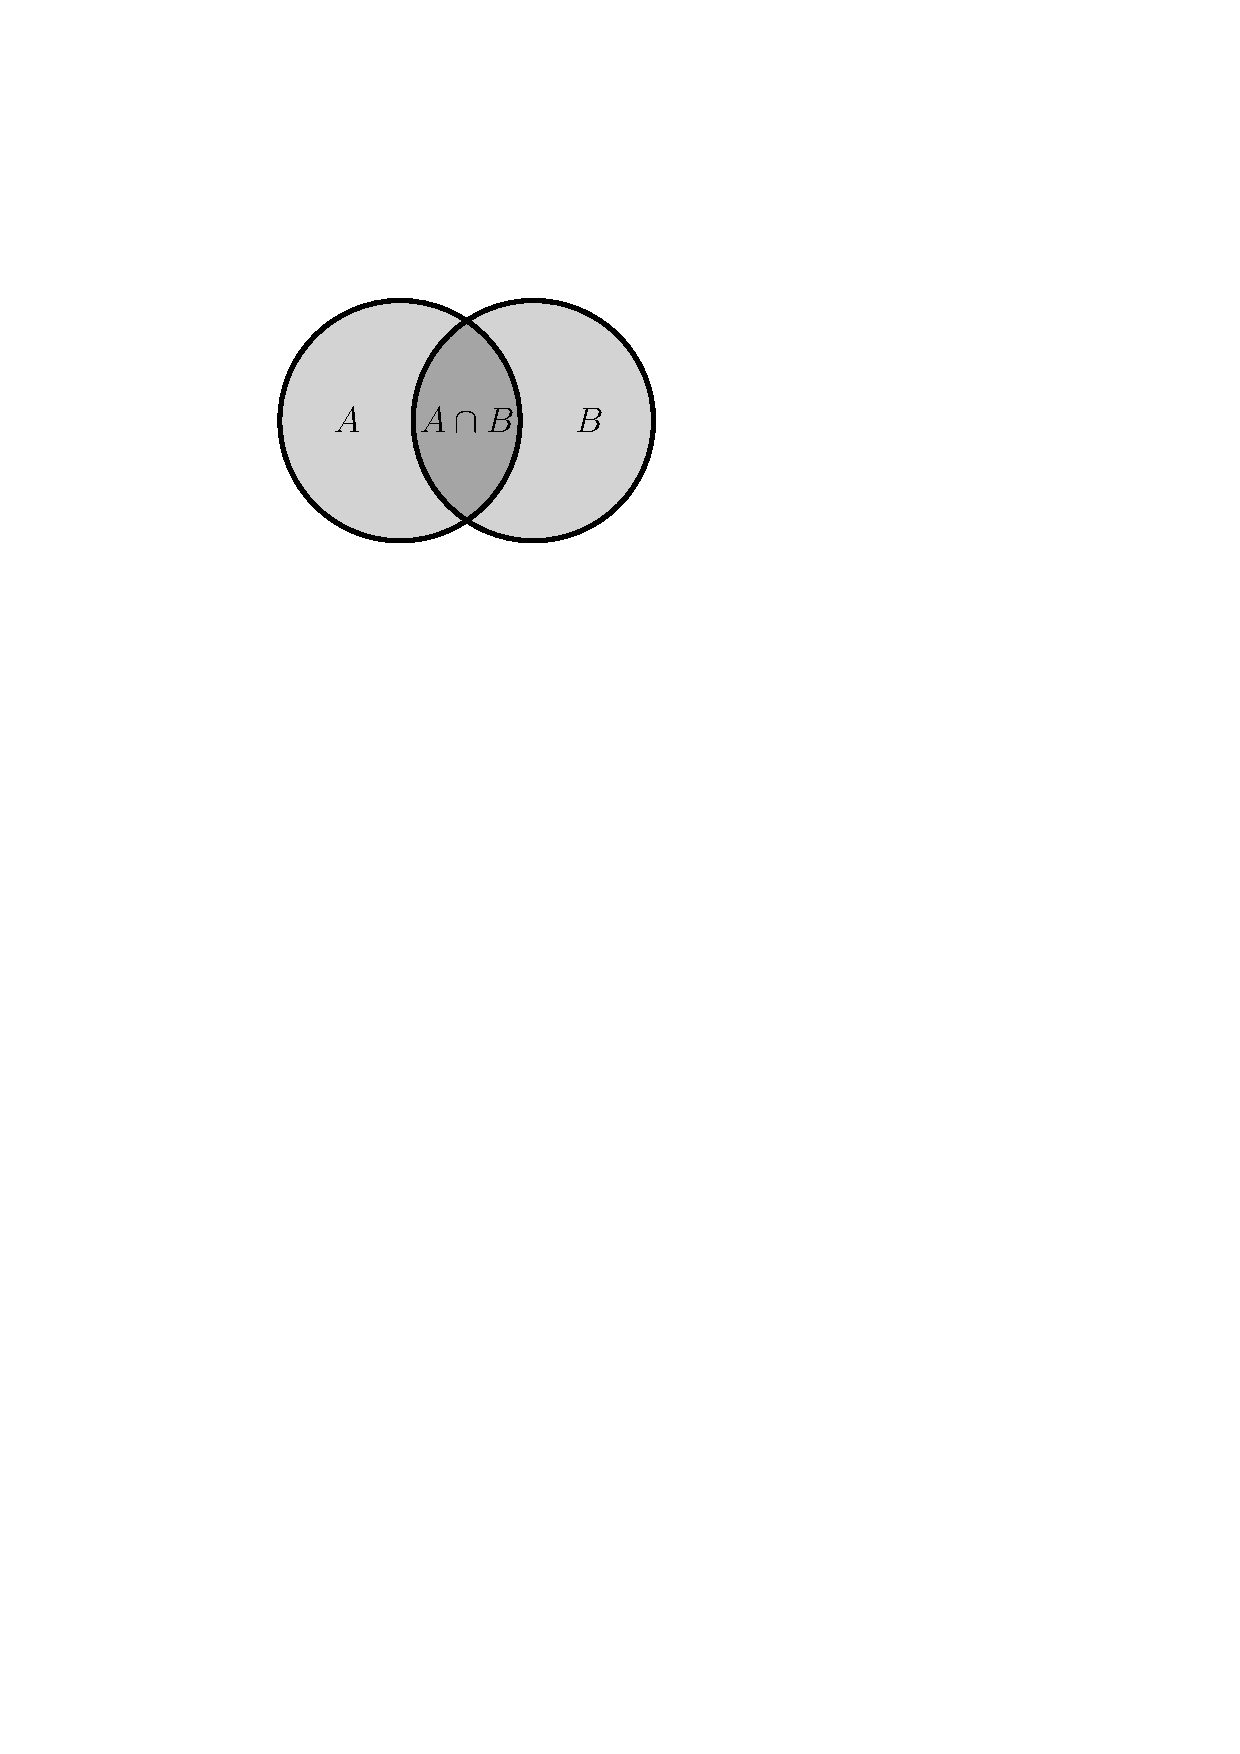
\includegraphics[scale=.5]{02_higher_combinatorics/pics/a_cut_b.pdf}
  \caption{When adding $|A|$ and $|B|$, the elements of $A \cap B$ will be counted twice.}
\end{figure}

In order to calcucate the cardinality of $|A \cup B|$ correctly we have to substract
$|A \cap B|$ from $|A| + |B|$:
\[
  |A \cup B| = |A| + |B| - |A \cap B|
\]

Now let's consider 3 overlapping sets $A$, $B$ and $C$. By simply adding up the cardinalities
$|A \cup B \cup C| = |A| + |B| + |C|$ once again many elements are double- or triple-counted:

\begin{figure}[htb]
  \centering
  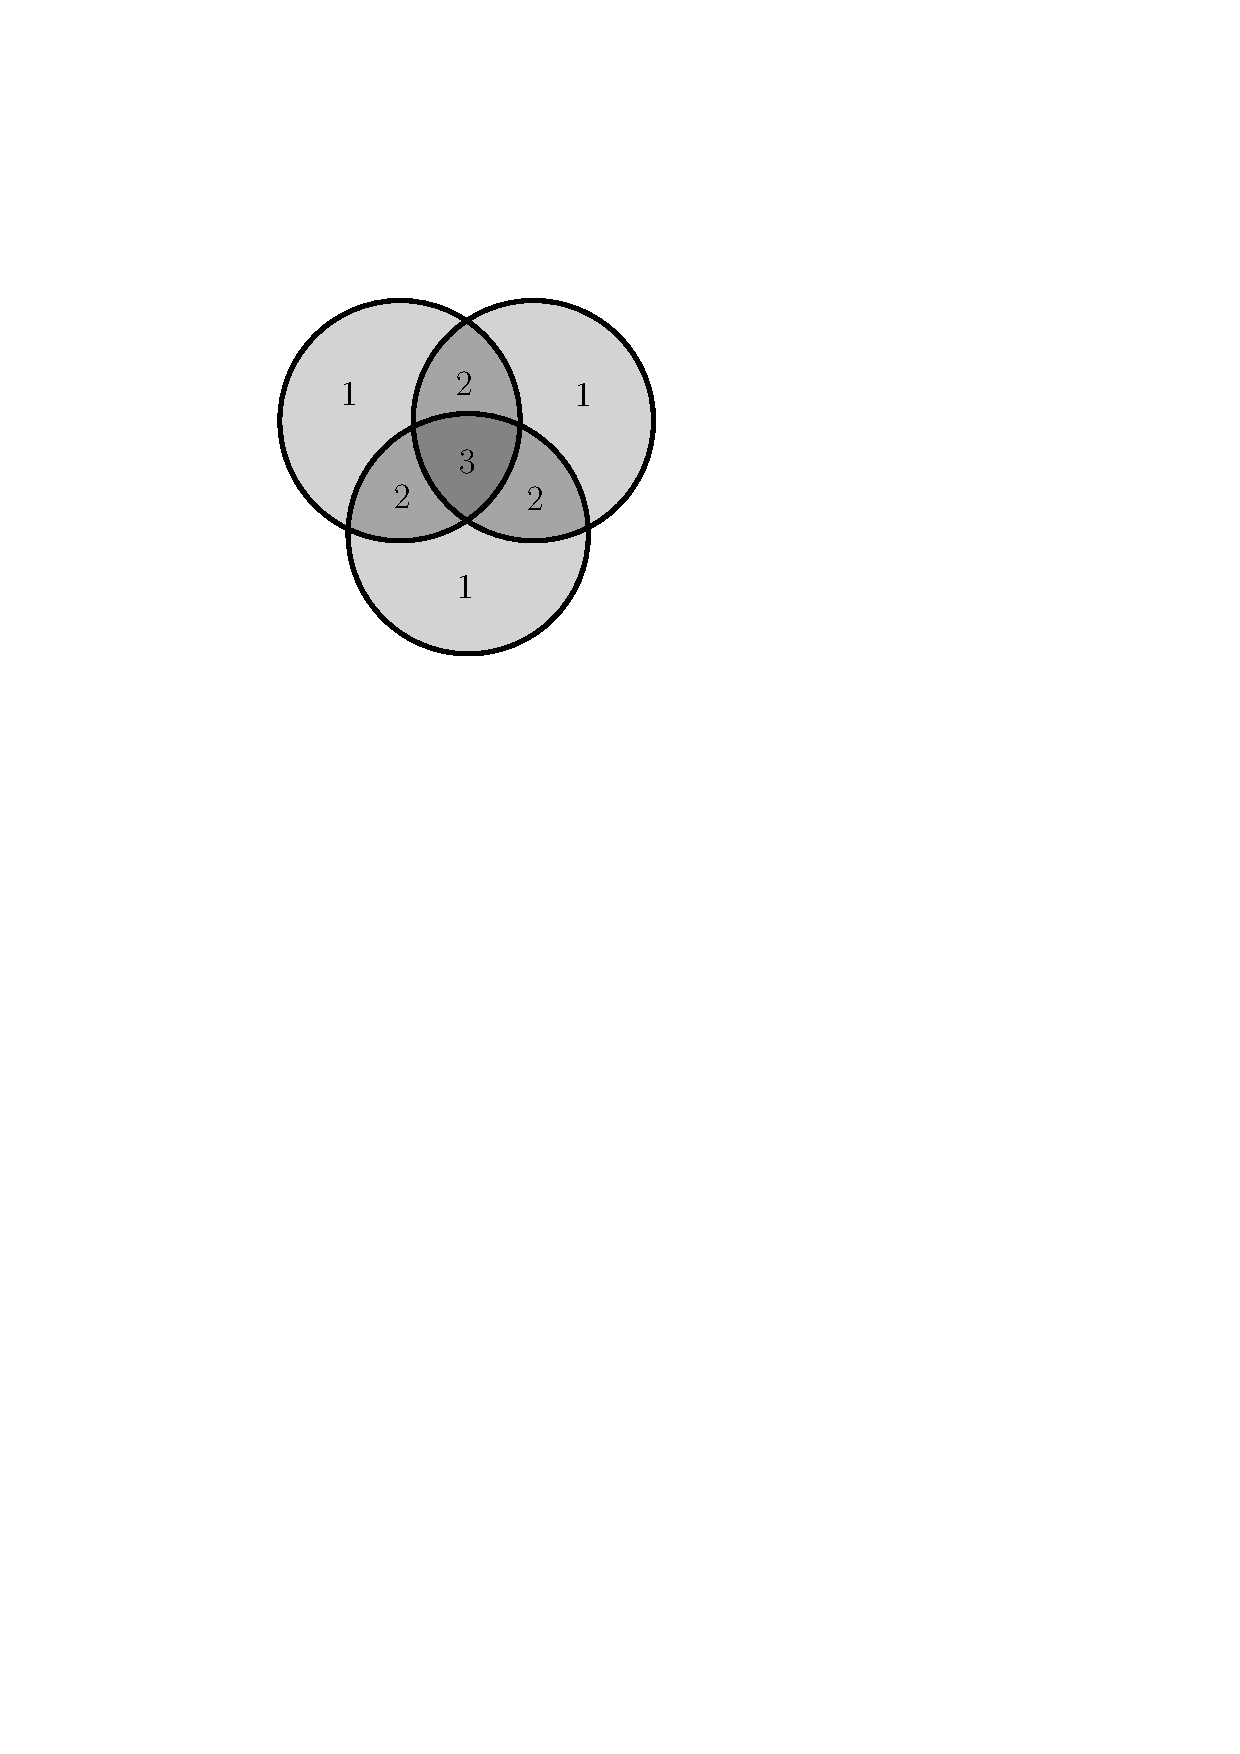
\includegraphics[scale=.5]{02_higher_combinatorics/pics/a_cut_b_cut_c.pdf}
  \caption{The numbers state, how often a certain area of $A \cup B \cup C$ has been counted by simply adding up $|A| + |B| + |C|$.}
\end{figure}

By substracting the number of elements of the cuts that were counted twice (namly $A \cap B$, $B \cap C$ and $C \cap A$) from $|A| + |B| + |C|$
we observe, that we now neglect the cut $A \cap B \cap C$ (because it had been counted 3 times before and we substract it's elements three times):

\begin{figure}[htb]
  \centering
  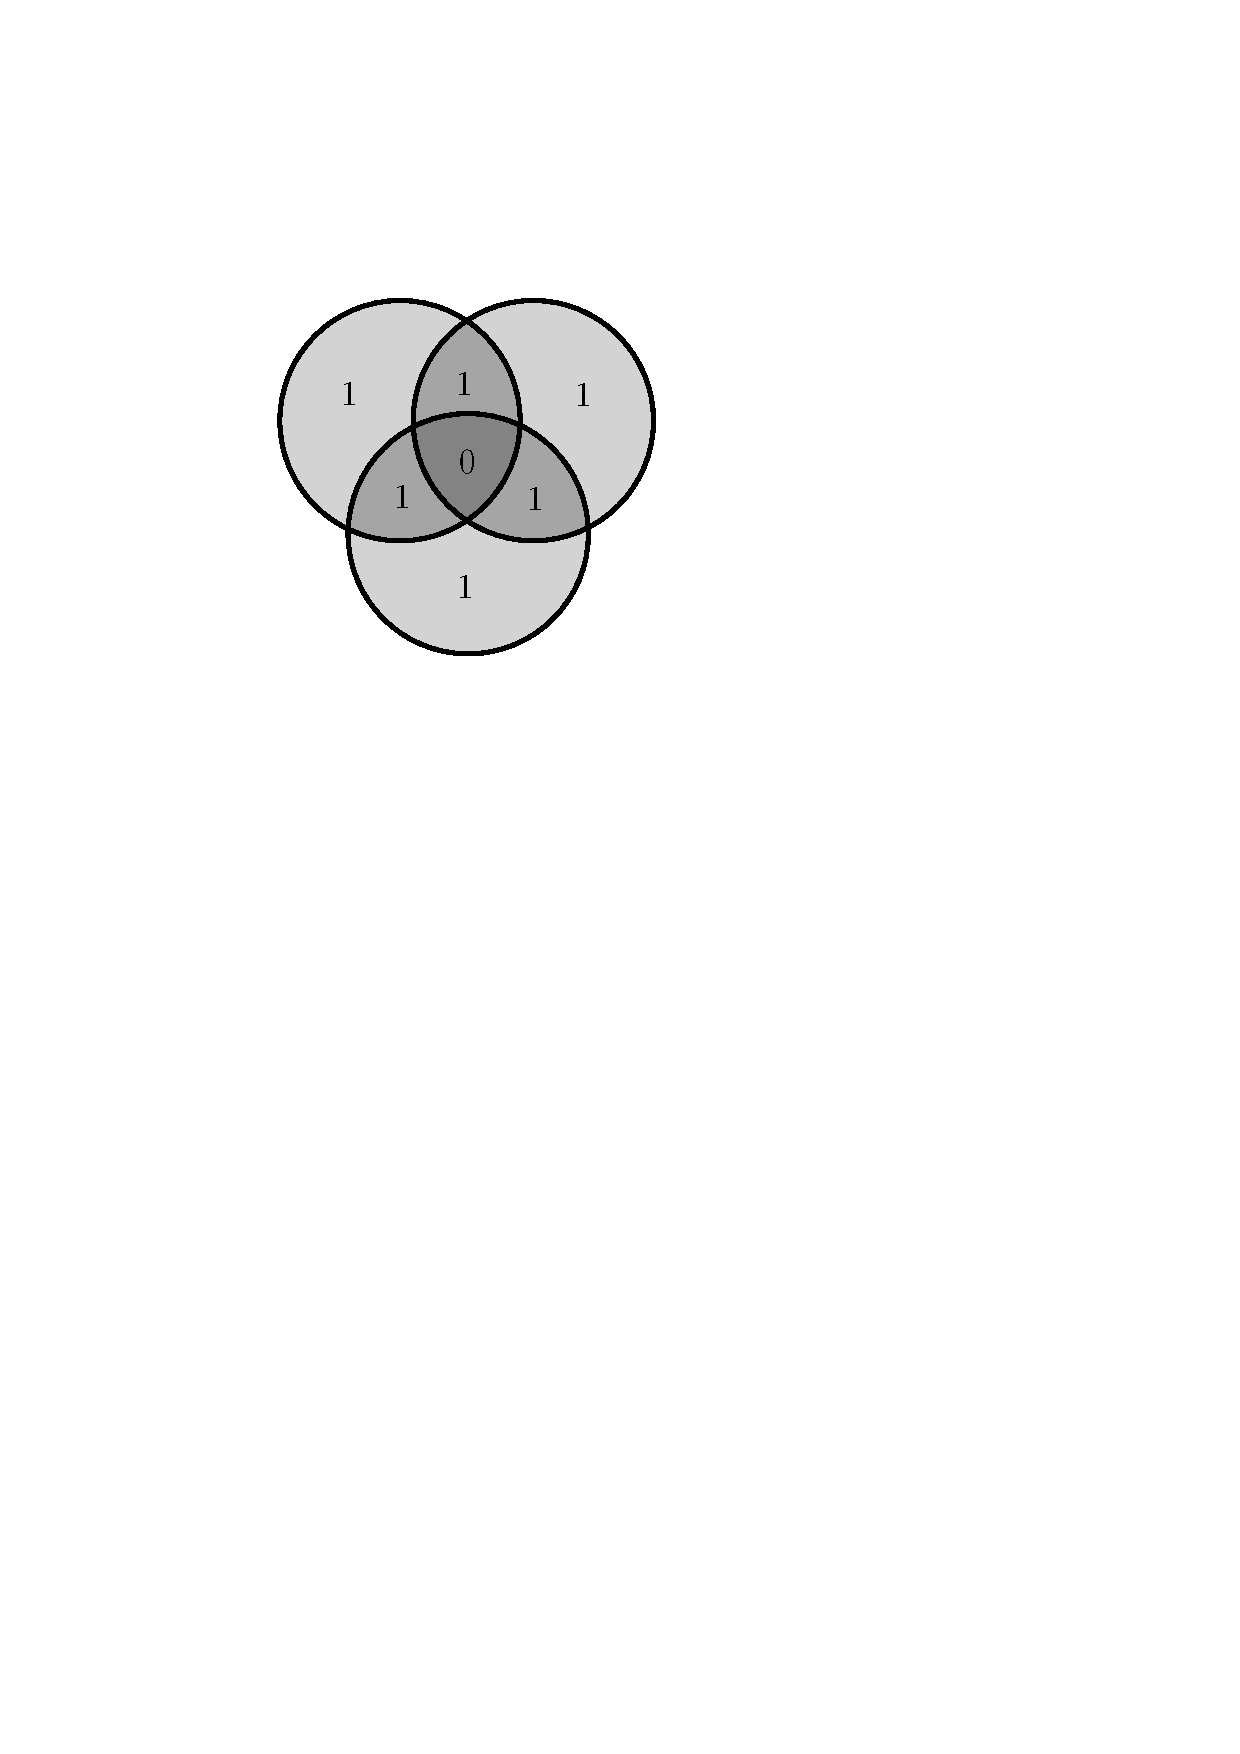
\includegraphics[scale=.5]{02_higher_combinatorics/pics/a_cut_b_cut_c_2.pdf}
  \caption{The numbers state, how often a certain area of $A \cup B \cup C$ has been counted by using the equation $|A| + |B| + |C| - |A \cap B| - |B \cap C| - |C \cap A|.$}
\end{figure}

So we have to add the number of elements of this cut again to get the correct number of elements in $A \cup B \cup C$.
All in all we get:

\[
  |A \cup B \cup C| = |A| + |B| + |C| - |A \cap B| - |B \cap C| - |C \cap A| + |A \cap B \cap C|
\]


With pairwise disjoint sets, we know that

\begin{align*}
  |A_1\cup \cdots\cup A_n| &= |A_1| + \ldots + |A_n|.\\
  |A_1\cup \cdots\cup A_n| &=
    \sum_{\varnothing\neq I\subseteq\{1,\ldots,n\}}
      (-1)^{|I|+1}
      \left|
        \bigcap_{i\in I} A_i
      \right|
\end{align*}

If we have a universe $A$ such that
\[
  A_1,\ldots,A_n \subseteq A
\]then

\begin{align*}
  |A\setminus \bigcup\limits_{i=1}^m A_i| &=
  |A| + \sum_{\varnothing\neq I\subseteq\{1,\ldots,n\}}
    (-1)^{|I|}
    \left| \bigcap_{i\in I} A_i \right| \\
  &= \sum_{I\subseteq\{1,\ldots,n\}}
    (-1)^{|I|}
    \left| \bigcap_{i\in I} A_i \right| \\
\end{align*}
\dots if you presume that the intersection of ``nothing'' is ``everything'' (A)

\subsection{Counting sets}

Finite Set $A = \{a_1, \ldots, a_n\}$, $n$-element-set or $n$-set

A \dt{counting set} is a set $A = \{1, 2, \ldots, n\}$

\begin{enumerate}
  \item number of permutations: $n!$
  \item number of $k$-subsets: ${n\choose k}$
  \item number of ordered $k$-subsets: $k! {n\choose k}$
  \item number of $k$-multisets: $b_1, \ldots, b_k \in A$, the order doesn't matter, but we are allowed to choose a element several times $\implies$ ${n +k-1 \choose k}$
\end{enumerate}

There is a mapping $f$ that maps the
\[
  \text{$k$-multiset}
  \subseteq A:
  b_1 ≤ \ldots ≤ b_k
\]
to the
\[
  \text{$k$-subset}
  \subseteq \{1,2,\ldots,n+k-1\}:
  b_1 < b_2+1 < \ldots < b_k+k-1.
\]

\begin{enumerate}
  \setcounter{enumi}{4}
  \item number of arrangements of a multiset: $\{b_1, b_1, \ldots , b_2, b_2,\ldots, b_2, \ldots, b_m, b_m, \ldots b_m\}$
\end{enumerate}

$b_1$ appears $k_1$ times, ...; $n$ in total

Permutations of this multiset:
$\frac{n!}{k_1! k_2! \ldots k_m!}$

\begin{enumerate}
  \setcounter{enumi}{5}
  \item number of ordered $k$-multisets over $A$: $n^k$ \\
  (we take a fixed number of positions $k$ and for each position choose any element from $A$)
\end{enumerate}

Remember:
\begin{compactitem}
  \item $\sum_{k=0}^n {n\choose k} = 2^n$
  \item Pascal's triangle
  \item ${n\choose k} + {n\choose k+1} = {n+1 \choose k+1}$
  \item $\sum_{m=0}^n {m\choose k} = {n+1 \choose k+1}$
  \item $\sum_{k=0}^n {m+k \choose k} = {m+n+1 \choose n}$
\end{compactitem}

\[
  \forall x,y\in \mathbb{C}
  \forall n\in \mathbb{N}
  (x+y)^n = \sum_{k=0}^n {n\choose k} x^k y^{n-k}
\]

$b_1, \ldots, b_k$ \; ${n \choose k} = \frac{n(n-1) \ldots (n-k+1)}{k!}$

\textbf{Definition (Extension to complex numbers).}
\index{binomial coefficient!for complex numbers}
Let $x\in \mathbb{C}, k\in\mathbb{N}$. Then we can define
\[
  {x\choose k} = \frac{
    x (x-1) \ldots (x-k+1)
  }{
    k!
  }
\]

\Lemma.
\[
  \forall k \in \mathbb{Z}, \forall x\in \mathbb{C}:
  {x\choose k} = {x-1 \choose k-1} + {x-1 \choose k}
\]
(with ${x \choose k} = 0$ for $k < 0$).

\Theorem. (Vandermonde's theorem).
\[
  {x+y \choose n} = \sum_{k=0}^{n} {x\choose k} {y\choose n-k},
  \forall n \in \mathbb{N}, \forall x,y \in \mathbb{C}
\]

\Proof.
Assume $x,y\in \mathbb{N}$. $X,Y$ sets: $X\cap Y=\varnothing, |X|=x, |Y|=y$.

Then the left-hand side
${x+y \choose n}$
is the number of $n$-subsets of $X\cup Y$.

Choose any $n$-subset $A\subseteq X\cup Y$.
Then $A$ can be decomposed like this:
\begin{gather*}
  A = (A\cap X)\cup (A\cap Y) \\
  |A\cap X| = k, |A\cap Y| = n-k
\end{gather*}

number of unions of shape right hand side of (*) $\left(={x+y \choose n} \right)$

\[
  \sum_{k=0}^n {x\choose k} {y\choose n-k}
\]

left hand side:
\[
  \sum_{i\in I} p_i (x) y^i
  = \sum \widetilde p_i (x) y^i
\]

lets assume $x\in \mathbb{N}$ and is fixed, then
\[
  Q_1(y) = Q_2(y) \; \forall y \in \mathbb{N}
  \implies \forall y\in \mathbb{C}
  p_i(x) = \widetilde p_i(x) \; \forall x \in \mathbb{N}
\]

\subsection{Stirling numbers}
Assume we have a set $A = \{1,2,3, \ldots ,n\}$
, permutation $\pi\in S_n$.
$S_n$ is the symmetric group; $|S_n| = n!$

We can represent $\pi$ as follows:
\[
  \begin{pmatrix}
    1&2&3&\cdots&n \\
    \pi(1)&\pi(2)&\pi(3)&\cdots&\pi(n) \\
  \end{pmatrix}
\]

2-line representation:
\[
  \begin{pmatrix}
    1&2&3&4&5&6&7 \\
    4&6&3&1&7&5&2 \\
  \end{pmatrix}
\]
The second line is also called the word representation.

Cycle representation:
$(1 4) (2 6 5 7) (3)$
Fixpoints can be omitted, so this is the same as $(14)(2657)$.

We can do calculations with permutations.

$(12)\in S_7 \implies (12)(3)(4)(5)(6)(7)$

A transposition is a permutation of just 2 elements.

Take $(12),(13)\in S_7$. Then $(12)\circ (13) = (132)$.

Every $\pi\in S_n$ can be written as a product of cycles, even as a product of transpositions (but not unique).

e.g. $(14)(2657) = (14)(27)(25)(26)$.

Of course, the order within a cycles does not matter:
$(2657)=(5726)$.

Canonical representation: generated from 2-line representation, smallest element comes first.
If additionally you start with the cycle with the largest last element first, you could even omit parentheses.

\begin{definition}
Let
\[
  s_{n,k} = \text{number of permutations of an $n$-set $A$ which have $k$ cycles}
\]
Then $s_{n,k}$ are the \dt{Stirling numbers of the first kind}.
(Fixpoints count as a cycle as well.)
\end{definition}

\Remark.
\begin{gather*}
  s_{n,1} = (n-1)! \\
  s_{n,n-1} = {n\choose 2} \\
  s_{n,n} = 1 \\
  s_{n,0} = s_{k,0} = 0 \quad n,k ≥ 1 \\
  s_{0,0} := 1 \\
  \sum_{k=0}^{n} s_{n,k} = n!
\end{gather*}

It doesn't matter where we start the cycle, just the order of the cycle needs to stay. $(3 2 6 5 7 1 4) = (6 5 7 1 4 3 2)$

\Theorem.
\[
  \forall n,k > 0:\;
  s_{n,k} = s_{n-1,k-1} + (n-1)s_{n-1,k}
\]

\Proof.
Take a permutation
$\pi = (1 \ldots )(\ldots) \ldots (\ldots) \in S_n \text{, with $k$ cycles}$.

How many such permutations are there?

\begin{compactitem}
  \item If $1$ is a fixed point: $s_{n-1, k-1}$.

  \item If $1$ is not a fixed point, start with a permutation of $n-1$ elements and add the element $1$ to one of the cycles. We can insert it before any of the $n-1$ elements, thus we get
$(n-1) s_{n-1,k}$ possibilities.
\end{compactitem}

\Remark.
Signed Stirling numbers of the first kind:
\[
  c_{n,k} = (-1)^{n+k} s_{n,k}
\]

\begin{definition}
Set partitions:
Take a set $A=\{1,2, \ldots, n\}$
and decompose it such that
\[
  A = A_1 \cup A_2 \cup \cdots\cup A_k
  \quad
  \forall i\neq j: A_i \cap A_j = \varnothing
\]
Then
\[
  S_{n,k} = \text{number of set partitions of $A$ with $k$ blocks}
\]
are the \dt{Stirling numbers of the second kind}.
\end{definition}

\textbf{Example.}
Set $A = \{1,2,3,4\}$
\begin{align*}
  \text{number of 1-partitions }= 1 &= S_{4,1}\\
  \text{number of 2-partitions }= 7 &= S_{4,2}\\
  \text{number of 3-partitions }= 6 &= S_{4,3}\\
  \text{number of 4-partitions }= 1 &= S_{4,4}
\end{align*}

\Remark.
\begin{align*}
  S_{n,1} &= S_{n,n} = 1 \\
  S_{n,2} &= 2^{n-1}-1 \\
  S_{n,n-1} &= {n\choose 2} \\
  S_{0,0} &:= 1 \\
  S_{n,0} &= S_{0,k} = 0
    \quad\forall n,k ≥ 1
\end{align*}

\Theorem.
\[
  S_{n,k} = S_{n-1,k-1} + k S_{n-1,k}
\]

\Proof.
If $\{1\}$ is a block:
\[
  S_{n-1,k-1}
\]
If $\{1\}$ is not a block, it has to be element of one of the $k$ blocks:
\[
  k S_{n-1,k}
\]

\Theorem.
$\forall x\in \mathbb{C} \forall n ≥ 0:$
\begin{gather*}
  (x)_n
    := x(x-1)(x-2) \ldots(x-n+1)
    = \sum_{k=0}^{n} (-1)^{n+k} s_{n,k} x^k \quad ((x)_0:=1)
    \\
  x^n = \sum_{k=0}^{n} S_{n,k} (x)_k
\end{gather*}

\Remark.
$V_n = \{a_0 + a_1 x + \ldots + a_n x^n \mid a_i \in \mathbb{C} \}$ \\
$\{1,x,x^2, \ldots , x^n\}, \{1,(x)_1, (x)_2, \ldots ,(x)_n\}$ are bases of $V_n$ \\
$(V_n, +, \mathbb{C})$ vector space dim $V_n = n+1$

basis change:
\[
  (S_{m,k})_{m,k= 0, \ldots,n}
    ((-1)^{m+k} s_{m,k})_{m,k= 0, \ldots,n}
\]

\Proof.
\begin{align*}
  (x)_n
  &= (x)_{n-1} (x-n+1) \\
  &= (x-n+1) \sum_{k=0}^{n-1} (-1)^{n-1+k} s_{n-1,k} x^k \\
  &= \sum_{k=0}^{n-1} (-1)^{n-1+k} s_{n-1,k} x^{k+1}
    + (n-1)\sum_{k=0}^{n-1} (-1)^{n+k} s_{n-1,k} x^k \\
  &= \sum_{k=1}^n (-1)^{n+k} s_{n-1,k-1} x^k
    \quad + (n-1)\sum_{k=0}^{n-1} (-1)^{n+k} s_{n-1,k} x^k \\
  &= \sum_{k=0}^n (-1)^{n+k}
    (s_{n-1,k-1} + (n-1)s_{n-1,k}) x^k \\
  &= \sum_{k=0}^n (-1)^{n+k} s_{n,k} x^k \\
\end{align*}
